\documentclass[ignorenonframetext, professionalfonts, hyperref={pdftex, unicode}]{beamer}

\usetheme{Copenhagen}
\usecolortheme{wolverine}

%Packages to be included
%\usepackage{graphicx}

\usepackage[russian]{babel}
\usepackage[utf8]{inputenc}
\usepackage[T1]{fontenc}

%%\usepackage[orientation=landscape, size=custom, width=16, height=9.75, scale=0.5]{beamerposter}

\usepackage{textcomp}

\usepackage{beamerthemesplit}

\usepackage{ulem}

\usepackage{verbatim}

\usepackage{ucs}


\usepackage{listings}
\lstloadlanguages{bash}

\lstset{escapechar=`,
	extendedchars=false,
	language=sh,
	frame=single,
	tabsize=2, 
	columns=fullflexible, 
%	basicstyle=\scriptsize,
	keywordstyle=\color{blue}, 
	commentstyle=\itshape\color{brown},
%	identifierstyle=\ttfamily, 
	stringstyle=\mdseries\color{green}, 
	showstringspaces=false, 
	numbers=left, 
	numberstyle=\tiny, 
	breaklines=true, 
	inputencoding=utf8,
	keepspaces=true,
	morekeywords={u\_short, u\_char, u\_long, in\_addr}
	}

\definecolor{darkgreen}{cmyk}{0.7, 0, 1, 0.5}

\lstdefinelanguage{diff}
{
    morekeywords={+, -},
    sensitive=false,
    morecomment=[l]{//},
    morecomment=[s]{/*}{*/},
    morecomment=[l][\color{darkgreen}]{+},
    morecomment=[l][\color{red}]{-},
    morestring=[b]",
}

\author[Epam]{{\bf Epam}\\Low Level Programming Department}

%\institution[EPAM]{EPAM}
%\logo{\includegraphics[width=1cm]{logo.png}}


\title{Введение в GNU/Linux}


%%%%%%%%%%%%%%%%%%%%%%%%%%%%%%%%%%%%%%%%%%%%%%%%%
%%%%%%%%%% Begin Document  %%%%%%%%%%%%%%%%%%%%%%
%%%%%%%%%%%%%%%%%%%%%%%%%%%%%%%%%%%%%%%%%%%%%%%%%




\begin{document}

\begin{frame}
	\frametitle{}
	\titlepage
	\vspace{-0.5cm}
	\begin{center}
	%\frontpagelogo
	\end{center}
\end{frame}


%%%%%%%%%%%%%%%%%%%%%%%%%%%%%%%%%%%%%%%%%   
%%%%%%%%%% Content starts here %%%%%%%%%%
%%%%%%%%%%%%%%%%%%%%%%%%%%%%%%%%%%%%%%%%%

\section{Перенаправление ввода-вывода}
\mode<all>{

\begin{frame}{Конвееры}
%  \textbf{Цель} -- максимальная модульность: большое количество простых приложений, взаимодействующих друг с другом для решения задач
  \only<1>{
  \begin{center}
    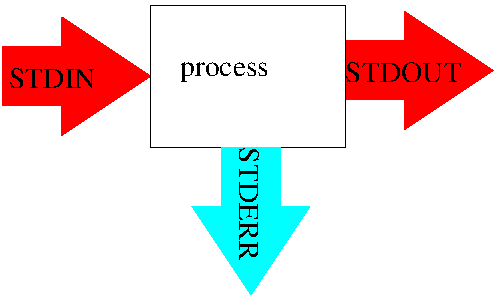
\includegraphics[width=1.2in]{../../slides/cmdline/process}
  \end{center}
  }
  \only<2>{
    \begin{center}
      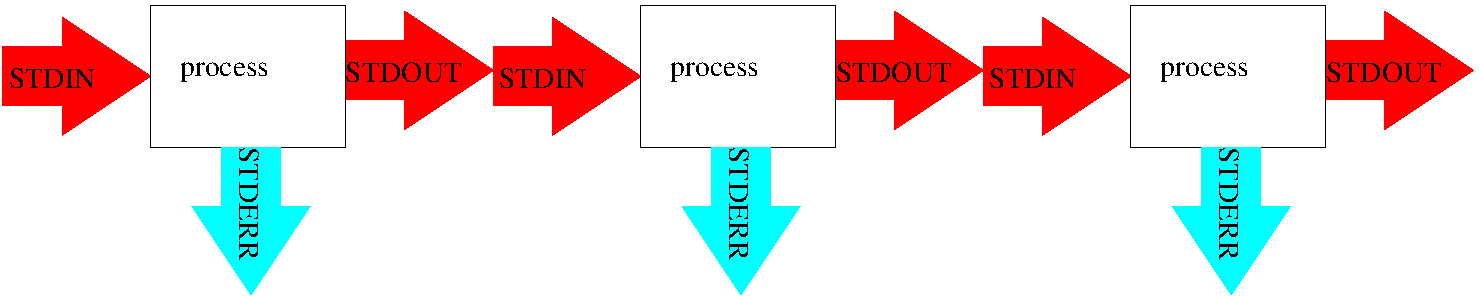
\includegraphics[width=3.6in]{../../slides/cmdline/processes}
    \end{center}
  }
  \begin{itemize}
    \item <1-> Каждое приложение открывает 3 стандартных файловых дескриптора stdin (fd 0), stdout(fd 1), stderr (fd 2)
    \item <2-> Приложения могут работать как фильтр из STDIN в STDOUT, можно объединять несколько приложений в конвейер
    \item <2-> Синтаксис {\tt <app1> | <app2>}
  \end{itemize}
\end{frame}
}
\mode<all>{\begin{frame}{Перенаправления в файл}

\begin{itemize}
  \item Перенаправление stdout 
    \begin{itemize}
      \item С созданием нового файла

        {\tt command > file}\\
		Например {\tt cat file1 file2 > file3}
      \item С дополнением существующего

		  {\tt command >\phantom{}>  file}
    \end{itemize}
    \pause
  \item Перенаправления stdin

    {\tt command < file}
    \pause
  \item Перенаправления stderr

    {\tt command1 2>\&1 | command2}

   {\tt command 1>file 2>\&1}

   {\tt command 2>file 1>\&2}
\end{itemize}

\end{frame}


}
\mode<all>{\begin{frame}[fragile]{Мультистрочный ввод (Here-документ)}

\begin{verbatim}
program <<LABEL
Тут
    много
	     строк
LABEL
\end{verbatim}

	\pause
	\begin{block}{Пример}
	Передадим несколько строк в COM-порт 1
\begin{lstlisting}[language=bash]
cat >/dev/ttyS0 <<E_O_F
ATZ
ATDT 8w0170123456
E_O_F
\end{lstlisting}
	\end{block}
\end{frame}
}

\section{Полезные команды}

\mode<all>{\begin{frame}{Дополнительный набор команд}
  \begin{itemize}
    \item {\tt cat} - Вывод файла в stdout, соединение нескольких файлов в stdout
    \item {\tt wc} - подсчет статистики символов в файле или в stdin 
    \item {\tt sort} - сортировка строк файла
    \item {\tt uniq} - объединение одинаковых строк в одну
    \item {\tt tr} - замена набора символов
    \item {\tt less} - программа-пейджер
    \item {\tt grep} - поиск строк, соответствующих регулярному выражению
    \item {\tt cut} - выделение полей из строк stdin
    \item {\tt awk} - небольшой язык программирования (также полезен для выделения полей)
  \end{itemize}
\end{frame}

\begin{frame}[fragile]{Некоторые примеры использования}
\begin{lstlisting}[language=bash]
cat /proc/1/environ | tr '\0' '\n' | less
ls  | wc -l # подсчет числа файлов
man uniq | tr  '[:space:]' '\n' | sort | uniq -c | sort -n | less # подсчет количества слов в тексте man uniq
history | wc -l # подсчет ранее введенных команд
cat /etc/udev/rules.d/* | wc -l
ls -s *.jpg | awk 'BEGIN{s=0};/^[ ]*[0-9]/{s+=\$1};END{print s}' 
\end{lstlisting}
  \pause
  \begin{block}{Упражнение}
    Посчитать статистику использования команд в history
  \end{block}
\end{frame}

\begin{frame}{Дополнительный набор команд для работы с текстом}
	\begin{itemize}
	  \item {\tt head} -- вывести первые строки
	  \item {\tt tail} -- вывести последние строки
		\begin{itemize}
			\item {\tt -f} -- отслеживать добавление данных в файл 
		\end{itemize}
	  \item {\tt tee} -- копировать стандартный вывод в файл
	  \item {\tt grep} -- печать текста, соответствующего шаблону
		\begin{itemize}
			\item {\tt -i}	
			\item {\tt -v}
			\item {\tt -o}
		\end{itemize}
	\end{itemize}
\end{frame}

}

\subsection{Архиваторы}
\mode<all>{\begin{frame}[fragile]{Архивация}
	\begin{block}{Архивация: tar}
		\begin{itemize}
			\item {\tt -c} -- создать архив
			\item {\tt -x} -- извлечь из архива
				\begin{itemize}
					\item {\tt -C} -- перейти в директорию
					\item {\tt -{}-strip-components=N} -- пропустить N уровней
				\end{itemize}
			\item {\tt -f} -- запись в файл
		\end{itemize}
	\end{block}

	\begin{block}{Сжатие: gzip, bzip, xz}
		\begin{itemize}
			\item {\tt -[1-9]} -- изменить уровень сжатия
			\item {\tt -d} -- распаковать
			\item {\tt -c} -- вывод на консоль
		\end{itemize}
		\begin{verbatim}
dd if=/dev/sda bs=1M count=1 | gzip -c > backup.gz
		\end{verbatim}
	\end{block}

\end{frame}

\begin{frame}[fragile]{Архивация: примеры}

	Создать сжатый архив:
	\begin{verbatim}
tar -czf archive.tar.gz *
	\end{verbatim}
	\pause
	Распаковать сжатый архив в директорию {\tt /tmp}:
	\begin{verbatim}
tar -C /tmp/ -xzf archive.tar.gz 
	\end{verbatim}
	\pause
	Создать сжатый архив:
	\begin{verbatim}
tar -czf archive.tar.gz *
	\end{verbatim}
	\pause
	Создать копию текущей директории в директории {\tt /tmp/copy/}:
	\begin{verbatim}
tar -c * | tar -C /tmp/copy -x
tar -cf - * | tar -C /tmp -xf -
	\end{verbatim}
	\pause
	Создать копию текущей директории на другом хосте:
	\begin{verbatim}
HostDest: netcat -l 2222 | gzip -dc | tar -C /tmp/copy/ -x
HostSrc:  tar -c * | gzip -9 | netcat HostDest 2222
	\end{verbatim}
\end{frame}
}

\subsection{find и xargs}
\mode<all>{\begin{frame}[fragile]{Поиск файлов}
	\begin{block}{find}
		\begin{itemize}
			\item {\tt -type} -- тип файлового объекта
			\item {\tt -size} -- размер
			\item {\tt -maxdepth} -- глубина рекурсии
			\item {\tt -exec} -- выполнить команду
			\item {\tt -printf} -- форматированный вывод
		\end{itemize}
	\end{block}

	\begin{block}{Примеры}
		\begin{verbatim}
find /etc -type f -size +100k  -exec ls -l {} \;
		\end{verbatim}

		\begin{verbatim}
find -type d -user altlinux
		\end{verbatim}
	
	\end{block}
\end{frame}

\begin{frame}[fragile]{xargs}
	\begin{block}{xargs}
			Утилита для создания и запуска команд из стандартного потока ввода:
		\begin{verbatim}
xargs [options] command [command options]
		\end{verbatim}

		\begin{itemize}
			\item {\tt -d} -- разделитель
			\item {\tt -0} -- null-terminated строки
			\item {\tt -I text} -- подстановка
			\item {\tt -n N} -- максимальное количество аргументов
			\item {\tt -P N} -- максимальное количество процессов
		\end{itemize}

	\end{block}
\end{frame}

\begin{frame}[fragile]{xargs}
	\begin{block}{Примеры}
		\begin{verbatim}
find /etc -type f -size -100k | xargs tar -czf /tmp/archive-100k.tar.gz
		\end{verbatim}

		\begin{verbatim}
find /etc -type f | xargs -I {} echo "Найден {} файл"
		\end{verbatim}

		\begin{verbatim}
find . -type f -name "*.mp3" -print0 | xargs -0 -n 1 -P 0 -I mp3 avconv -i mp3 mp3.ogg
		\end{verbatim}
	
	\end{block}
\end{frame}


}

\subsection{Редакторы}
\mode<all>{\begin{frame}{Редакторы}
	\begin{itemize}
		\item Интерактивные
			\begin{itemize}
				\item vi
					\begin{itemize}
						\item Есть почти везде
					\end{itemize}
				\item vim
				\item emacs
			\end{itemize}
		\item Поточные
			\begin{itemize}
				\item {\tt ed}
				\item {\tt sed}
				\item {\tt awk}
			\end{itemize}
	\end{itemize}
\end{frame}

\begin{frame}[fragile]{Метасимволы}
	\begin{block}{grep, sed, awk}
	\end{block}
	\begin{itemize}
		\item {\tt .} -- любой символ за исключением пустой строки
		\item {\tt *} -- любоe количество символов, которые стоят перед {\tt *}
		\item {\tt \^{}} -- начало строки
		\item {\tt \$} -- конец строки
		\item {\tt [...]} -- любой символ из заключенных в скобки
	\end{itemize}
\end{frame}

\begin{frame}[fragile]{sed}
	\begin{block}{Сценарии}
		{\tt [ addr [ ,  addr ] ] cmd [ args ]}
	\end{block}

	\tiny
	\begin{block}{Команды}
		\begin{itemize}
		  \item {\tt a, i} -- добавить строку после (перед) текущей
			  \begin{verbatim} who | sed -e 'a Text' \end{verbatim}
		  \item {\tt c} -- удалить строку и заменить на текст
			  \begin{verbatim} who | sed -e "/$USER/ c Юзверь" \end{verbatim}
		  \item {\tt d} -- удалить строку
			  \begin{verbatim} who | sed -e '2,4 d' \end{verbatim}
			  \begin{verbatim} who | sed -e '/pts/ d' \end{verbatim}
		  \item {\tt s} -- замена по регулярному выражению
			  \begin{verbatim} who | sed -e "s/$USER/Юзверь/g" \end{verbatim}
		\end{itemize}
	\end{block}
\end{frame}


}

\mode<all>\begin{frame}[fragile]{Вопросы?}
    \setcounter{tocdepth}{2}
    \tableofcontents

    \bigskip

    \hrulefill
    \begin{columns}
    \column{0.7\textwidth}
            \center{Материалы:}
            \url{https://yadi.sk/d/Ixp8kHfl3MipCq}
    \column{0.2\textwidth}
        \begin{center}
            
\includegraphics[width=0.7\textwidth]{url-qr-2017}
        \end{center}
    \end{columns}

    Исходники: \url{https://github.com/epam-llpd/linux_courses}

\end{frame}

\end{document}
